\documentclass{article}
\usepackage[OT1]{fontenc}
\usepackage[utf8]{inputenc}
\usepackage{amsthm,amssymb,amsmath}
\usepackage[a4paper, total={6.5in, 9in}]{geometry}
\usepackage[compact,explicit]{titlesec}
\usepackage[greek,english]{babel}
%\usepackage[iso-8859-7]{inputenc}
\usepackage[table]{xcolor}
%\usepackage{amsfonts}
%\usepackage{amsmath}
\usepackage{amssymb}
\usepackage{amsmath}
\usepackage{pgfplots}
\usepackage{tikz}
\usepackage{tikzscale}
\usepackage{array}
\usepackage{booktabs}
\usepackage{enumerate}
%\usepackage{color}
%AASFASFASF
\usepackage{empheq}
\usepackage{enumerate}
\usepackage{enumitem}
%\usepackage{gensymb}
\usepackage{graphicx}
\usepackage[space]{grffile}
\usepackage{ifthen}
%\usepackage{kerkis}
\usepackage{marginnote}
\usepackage{mathtools}
\usepackage{mdframed}
\usepackage{multirow}
%\usepackage{textgreek}
\usepackage{float}
\usepackage{slashbox}
\usepackage{listings}

\usepackage{caption}
\usepackage{afterpage}
\usepackage{forloop}
\usepackage{systeme}
\usepackage{cancel}
\usepackage{subcaption}
\usepackage{hyperref}
\usepackage{tikzsymbols}
\usetikzlibrary{calc}
\usepackage{changes}
\usepackage{cancel}
\setdeletedmarkup{\cancel{#1}}
%\usepackage{bbold}
%\newtheorem*{theorem}{Theorem}




\newcommand{\NN}{\mathbb{N}}
\newcommand{\ZZ}{\mathbb{Z}}
\newcommand{\RR}{\mathbb{R}}
\newcommand{\RRp}{\mathbb{R}^{+}}
\newcommand{\RRpp}{\mathbb{R}^{++}}
\newcommand{\QQ}{\mathbb{Q}}
\newcommand{\CC}{\mathbb{C}}
\newcolumntype{P}[1]{>{\centering\arraybackslash}p{#1}}

\newcommand{\tl}[1]{\textlatin{#1}}
\renewcommand\thesubfigure{(\roman{subfigure})}\usepackage{pgf, tikz}

\setlength{\arrayrulewidth}{1mm}
\setlength{\tabcolsep}{18pt}
\renewcommand{\arraystretch}{1.5}


\newcommand\blankpage{%
	\null
	\thispagestyle{empty}%
	\addtocounter{page}{-1}%
	\newpage}

\newcommand{\thewr}[1]{\mathrm{\ifthenelse{\equal{#1}{}}{}{#1,}\theta\epsilon\omega\rho}}
\newcommand{\peir}[1]{\mathrm{\ifthenelse{\equal{#1}{}}{}{#1,}\pi\epsilon\iota\rho}}
%\newcommand{\Upd}{\operatorname{U}^{\mathrm{M}}_{#1}}

\newlength\dlf
\newcommand\alignedbox[2]{
	% #1 = before alignment
	% #2 = after alignment
	&
	\begingroup
	\settowidth\dlf{$\displaystyle #1$}
	\addtolength\dlf{\fboxsep+\fboxrule}
	\hspace{-\dlf}
	\boxed{#1 #2}
	\endgroup
}

\setlist{  
	listparindent=\parindent%,
	%parsep=0pt
}

\hypersetup{
	colorlinks,
	linkcolor={red!50!black},
	citecolor={blue!50!black},
	urlcolor={blue!80!black}
}



%\let\thetitle\@title
%\let\theauthor\@author
%\let\thedate\@date

\DeclarePairedDelimiter\ceil{\lceil}{\rceil}

\DeclareMathOperator*{\argmax}{argmax} % thin space, limits underneath in display
\makeatother

\allowdisplaybreaks

%Η απόλυτη τιμή
\DeclarePairedDelimiter\abs{\lvert}{\rvert}


\renewcommand{\theenumi}{\roman{enumi}}
\begin{document}
	\greektext
	\captionsetup[figure]{labelfont={default},labelformat={default},labelsep=period,name={Σχήμα:}}
	\captionsetup[table]{labelfont={default},labelformat={default},labelsep=period,name={Πίνακας:}}
	\title{\tl{Assignment 2: Blob Detection}}						% Title
	\author{Μαυρογιώργης Δημήτρης, AM:2016030016\\Κολομβάκη Αφροδίτη, AM:2016030158\\Δελατόλας Θάνος, AM:2016030074}								% Author
	\date{\today}											% Date
	
	\makeatletter
	\let\thetitle\@title
	\let\theauthor\@author
	\let\thedate\@date
	\makeatother
	
	
	
	\begin{titlepage}
		\centering
		\vspace*{0.5 cm}
		\includegraphics[scale = 0.4]{../../Assignment 1/report/polytexneio-logo.png}\\[1.0 cm]	% University Logo
		\textsc{\LARGE Μηχανικη Όραση }\\[2.0 cm]	
		\rule{\linewidth}{0.2 mm} \\[0.4 cm]
		{ \huge \bfseries \thetitle}\\
		\rule{\linewidth}{0.2 mm} \\[1.5 cm]
		
		\begin{minipage}{0.6\textwidth}
			
			\begin{flushright} \large
				\theauthor\\
				
			\end{flushright}
			
			\begin{flushright} \large
				\tl{\thedate}\\
				
			\end{flushright}
			
		\end{minipage}\\[2 cm]
		
	\end{titlepage}	
	\newpage
	
	\section*{1. \tl{Introduction}}
	Σκοπός του αλγορίθμου \tl{scale-invariant feature transform (SIFT)} που χρησιμοποιείται ευρέως στη Μηχανική όραση, είναι να εντοπίσουμε και να περιγράψουμε κάποια τοπικά 
	χαρακτηριστικά στις ψηφιακές εικόνες, με απότερο στόχο να αναγωνρίσουμε δύο διαφορετικές λήψεις-περιοχές της ίδιας εικόνας. Για παράδειγμα, με βάση τις ίδιες περιοχές να 
	καταλάβει ο αλγόρισμος ότι πρόκειται για την ίδια εικόνα τραβηγμένη από διαφορετική γωνία. Πιο συγκεκριμένα, στη δεύτερη εργαστηριακή άσκηση κληθήκαμε να υλοποιήσουμε έναν \tl{Laplacian blob detector}. Ένας \tl{blob detector}
	είναι υπεύθυνος να υπολογίζει περιοχές στις ψηφιακές εικόνες οι οποίες έχουν διαφορετικά χαρακτηριστικά, δηλαδή διαφέρουν ως προς κάποιες ιδιότητες. Για παράδειγμα, κάποια 
	χαρακτηριστικά περιοχών είναι η φωτεινότητα της εικόνας ή και το χρώμα της. Επιπλέον, η μέθοδος που χρησιμοποιήσαμε για να υπολογίσουμε τα σημεία ενδιαφέροντος \tl{(key points)} 
	βασίζονται στα τοπικά ακρότατα, δηλαδή βασίζονται στην εύρεση τοπικών μεγίστων ή ελαχίστων της συνάρτησης.

	\ \\\\\\
	\section*{2. \tl{Implementation}}
	\begin{itemize}
		\item \textbf{\tl{Generate a Laplacian of Gaussian filter.}}\\\\ \noindent 
		Το \tl{Laplacian of Gaussian filter}  δημιουργήθηκε με τη συνάρτηση \tl{fspecial} με \tl{size} \tl{n X n pixels} όπου $n=2\cdot\tl{ceil}(3\cdot\sigma) +1$.  Το μέγεθος του φίλτρου καθορίζεται από το \tl{standard deviation} απο τη παραπάνω σχέση γιατί:
		\begin{itemize}
			\item Ο όρος $3\cdot \sigma$ προσεγγίζει το μέγεθος της διαφοράς δυο \tl{gaussian} φίλτρων
			\item Πολλαπλασιάζουμε με το 2 εφόσον οι εικόνες μας είναι \tl{2-D}.
			\item Προσθέτουμε 1 για να έχουμε περιττό μέγεθος φίλτρου. Ο λόγος που θέλουμε περιττό μέγεθος του φίλτρου είναι επειδή στην τελική εικόνα μετά τη συνέλιξη 
			έχουμε μια συμετρία στα \tl{pixel} κάτι που δε συμβαίνει όταν έχουμε ζυγό αριθμό καθώς τότε θα πρέπει να υπολογίσουμε και κάποια πιθανή \tl{distortion}.
		\end{itemize}
		\ \\
		\noindent 
		Γνωρίζουμε πως κανονικοποιούμε την \tl{Gaussian} πολλαπλασιάζοντας με $\sigma$ και εφόσον η \tl{Laplacian of Gaussian} είναι η δευτερη
		παράγωγος της \tl{Gaussian} κανονικοποιήται με τη διασπορά ($\sigma^2$). \\
		\item \textbf{\tl{Build a Laplacian scale-space.}}\\\\ \noindent 
		Αρχικά, υλοποιήσαμε την περίπτωση όπου εφαρμόζουμε \tl{downsampling} στις εικόνες των επιπέδων. Για κάθε επίπεδο $i > 1$ γίνεται \tl{downsample} της αρχικής εικόνας κατα $\frac{1}{k^{i-1}}$
		χρησιμοποιώντας τη συνάρτηση \tl{imresize}. Στη συνέχεια γίνεται συνέλιξη της \tl{downsampled} εικόνας με το φίλτρο με τη συνάρτηση \tl{imfilter}, ενώ αφού υπολογίσουμε το τετράγωνο της συνέλιξης επαναφέρουμε την εικόνα στις αρχικές της διαστάσεις έτσι ώστε στα επόμενα βήματα να μπορέσουμε να συγκρίνουμε ανα \tl{pixel} τα \tl{layers}.\\\\
		\noindent
		Επιπλέον υλοποιήσαμε τη δεύτερη περίπτωση όπου αυξάνουμε το μέγεθος του φίλτρου κρατώντας το μέγεθος της εικόνας σταθερό. Από τη διάλεξη η τυπική απόκλιση για κάθε επίπεδο $i$ υπολογίζεται από τη σχέση $\tl{scaled\_sigma} = \sigma \cdot k^{i-1}$. Tα υπόλοιπα βήματα που ακολουθήσαμε ήταν όμοια με την πρώτη πρείπτωση με μοναδική διαφορά ότι δεν χρειάστηκε \tl{upsample} στο τετράγωνο της συνέλιξης.
		\newpage		
		\item \textbf{\tl{Find the extrema in the scale-space.}}\\\\ \noindent
		Σε αυτό το στάδιο του αλγορίθμου βρίσκουμε τη μέγιστη τιμή ανάμεσα στους 26 γείτονες κάθε \tl{pixel}, όπου αυτοί οι γείτονες βρίσκονται σε 3 διαδοχικά επίπεδα. Τα μέγιστα σημεία αποτελούν τα \tl{key points}.\\\\
		\noindent
		
		Όσον αφορά τη διαδικασία που ακολουθήθηκε είναι η εξής: 
		\begin{itemize}
			\item Mε τη συνάρτηση \tl{ordfilt2} βρίσκουμε το μέγιστο \tl{pixel} μιας γειτονίας 3 \tl{x} 3 του ίδιου επιπέδου.
			\item Mε ένα \tl{for-loop} υπολογίζουμε το μέγιστο \tl{pixel} αλλά σε 3 διαδοχικά επίπεδα. 
		\end{itemize}
		\noindent
		Από το πρώτο βήμα παίρνουμε το μέγιστο 9 \tl{pixel} και σε συνδιασμό με το δεύτερο βήμα παίρνουμε το μέγιστο 3 \tl{x} 9 \tl{pixel}, δηλαδή ενός \tl{pixel (i,j)} και των 26 γειτόνων του.
		\item \textbf{\tl{Display the resulting circles at their characteristic scales.}}\\\\ \noindent
		Όσον αφορά το συγκεκριμένο βήμα, βρίσκουμε τη θέση στο επίπεδο κάθε κύκλου η οποία είναι η θέση του αντίστοιχου \tl{maxima} σημείου και υπολογίζουμε την ακτίνα του με βάση τη σχέση: $\sqrt(2)\cdot \sigma \cdot k^{i-1}$
	\end{itemize}

	\section*{3. Επιλογή παραμέτρων}
	Έπειτα απο δοκιμές καταλήξαμε στις τιμές:
	\begin{itemize}
		\item $\sigma = 2$ 
		\item \tl{threshold}=0.005
		\item \tl{layers}=15
	\end{itemize}
	\noindent
	Επιπλέον, βρήκαμε πως το κατάλληλο $k$ είναι $k=\sqrt{\sqrt{2}} \approx 1.2$. Όσον αφορά την επιλογή του $\sigma$, δεν επιλέξαμε τιμή 1,
	επειδή ναι μεν τα αποτελέσματα δεν ήταν και τόσο βέλτιστα αλλά ο χρόνος εκτέλεσης του αλγορίθμου ήταν πολύ μικρότερος. Επιπλέον, δεν 
	χρησιμοποιήσαμε κάποια μεγαλύτερη τιμή $\sigma$ καθώς ο χρόνος εκτέλεσης αυξανόταν αρκετά, ενώ παράλληλα δεν υπήρχε κάποια σημαντική 
	βελτίωση των αποτελεσμάτων. Τέλος, για το \tl{threshold} δεν επιλέξαμε κάποια μεγαλύτερη τιμή, γιατί δεν παρατηρούσαμε σημαντικές αλλαγές 
	ως προς συνολικό αριθμό κύκλων.
	\\\\\
	\section*{4. Σύγκριση}
	
	\begin{figure}[H]
		\begin{subfigure}[b]{0.37\textwidth}
			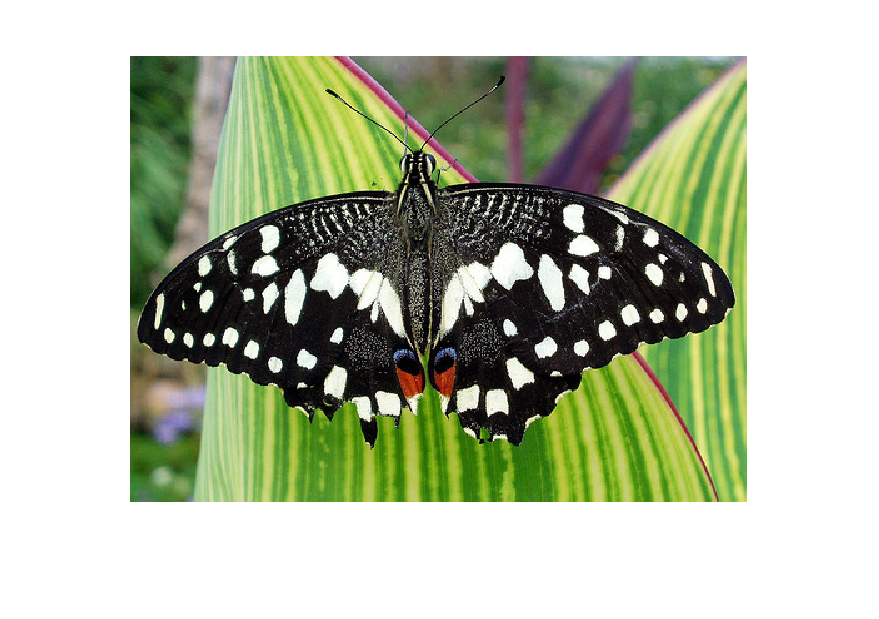
\includegraphics[width=\textwidth]{res/butterfly.eps}
			\caption{\tl{Orginal Image}}
		\end{subfigure}%
		\begin{subfigure}[b]{0.37\textwidth}
			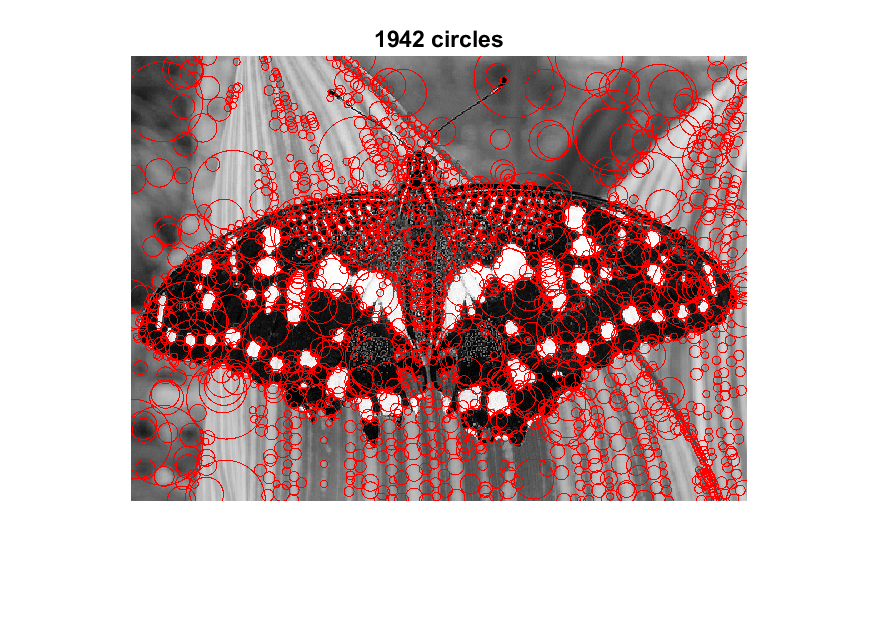
\includegraphics[width=\textwidth]{res/butterfly_blob_method2.eps}	
			\caption{\tl{Image Downsampling}}	
		\end{subfigure}%	
		\begin{subfigure}[b]{0.37\textwidth}
			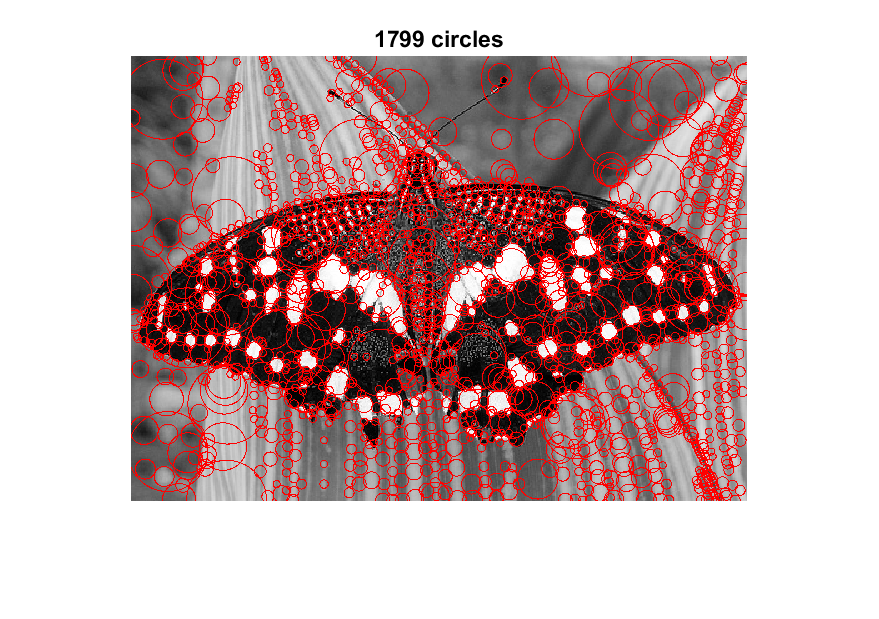
\includegraphics[width=\textwidth]{res/butterfly_blob.eps}	
			\caption{\tl{Filter Resizing}}	
		\end{subfigure}%	
	\end{figure}

	\begin{figure}[H]
		\begin{subfigure}[b]{0.37\textwidth}
			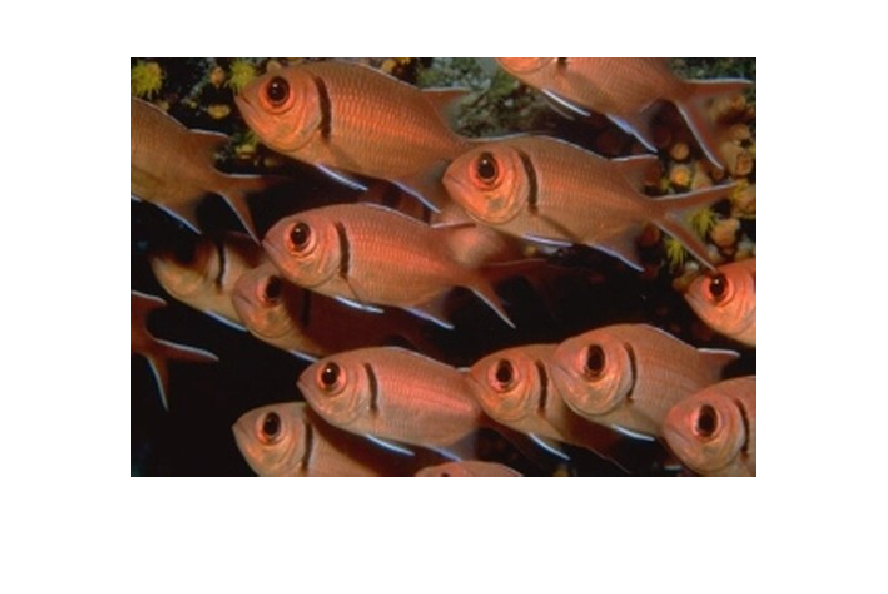
\includegraphics[width=\textwidth]{res/fishes.eps}
			\caption{\tl{Orginal Image}}
		\end{subfigure}%
		\begin{subfigure}[b]{0.37\textwidth}
			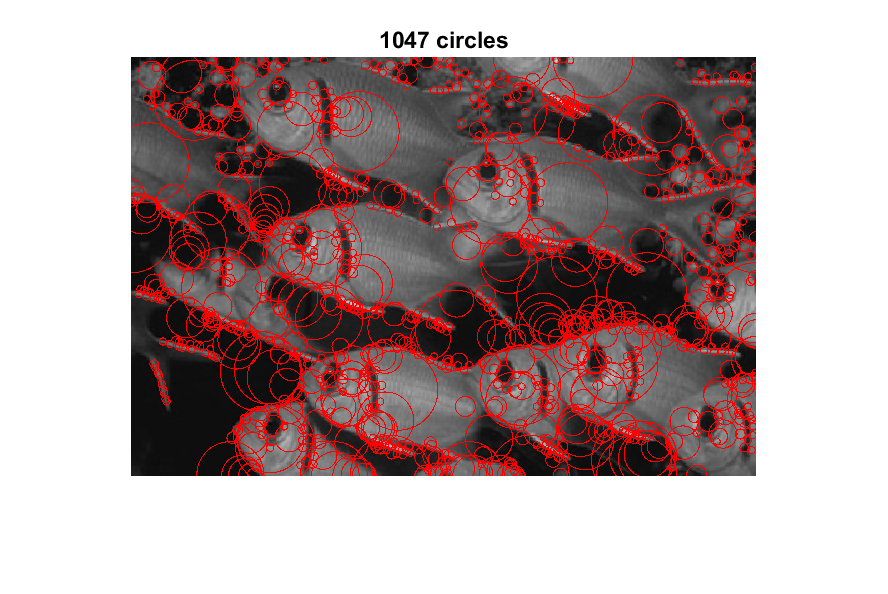
\includegraphics[width=\textwidth]{res/fishes_blob_method2.eps}	
			\caption{\tl{Image Downsampling}}	
		\end{subfigure}%
		\begin{subfigure}[b]{0.37\textwidth}
			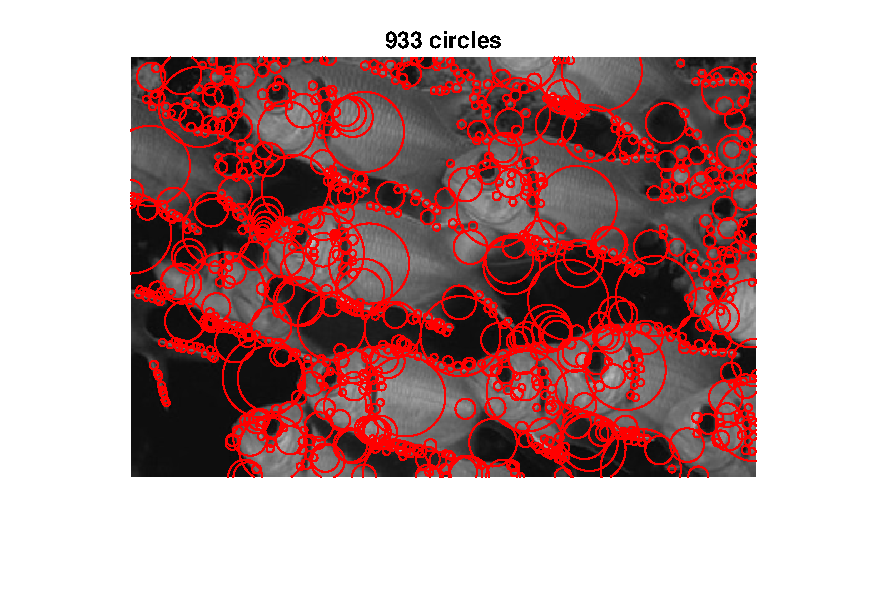
\includegraphics[width=\textwidth]{res/fishes_blob.eps}	
			\caption{\tl{Filter Resizing}}	
		\end{subfigure}%	
	\end{figure}

	\begin{figure}[H]
		\begin{subfigure}[b]{0.37\textwidth}
			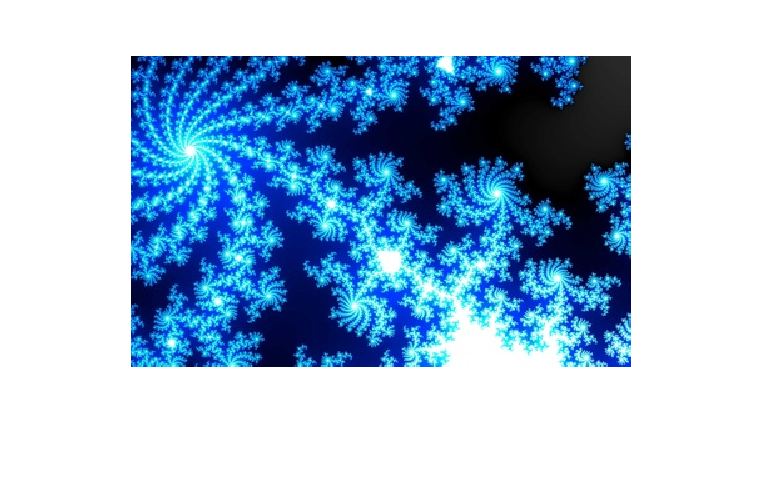
\includegraphics[width=\textwidth]{res/snowflakes.eps}
			\caption{\tl{Orginal Image}}
		\end{subfigure}%
		\begin{subfigure}[b]{0.37\textwidth}
			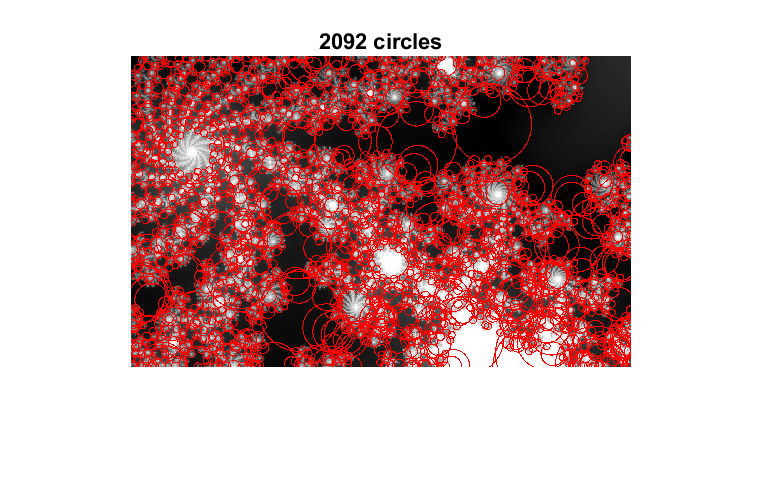
\includegraphics[width=\textwidth]{res/snowflakes_blob_method2.eps}	
			\caption{\tl{Image Downsampling}}	
		\end{subfigure}%
		\begin{subfigure}[b]{0.37\textwidth}
			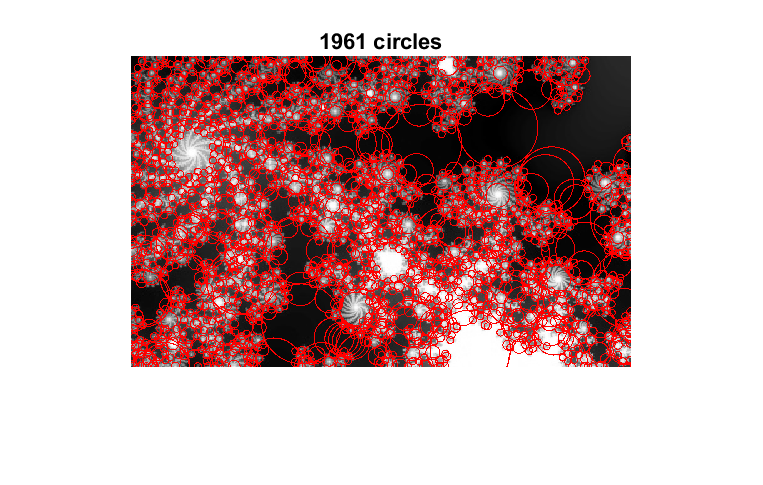
\includegraphics[width=\textwidth]{res/snowflakes_blob.eps}	
			\caption{\tl{Filter Resizing}}	
		\end{subfigure}%	
	\end{figure}
	
	\begin{figure}[H]
		\begin{subfigure}[b]{0.37\textwidth}
			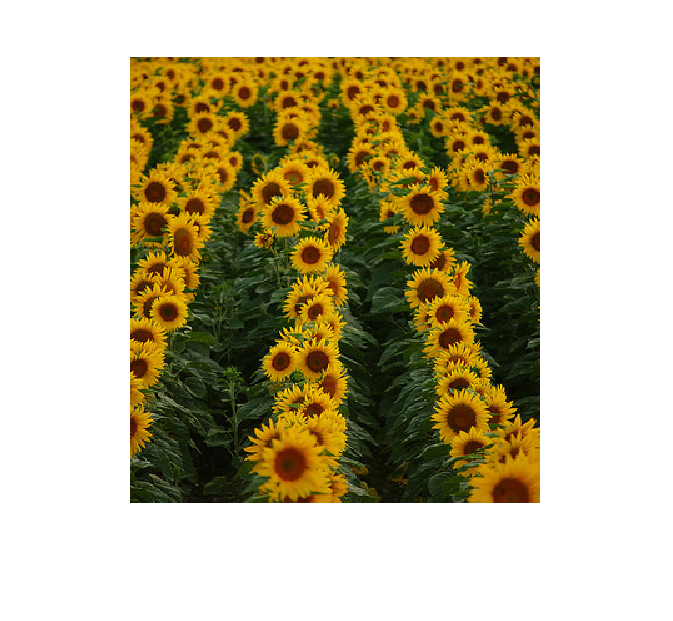
\includegraphics[width=\textwidth]{res/sunflowers.eps}
			\caption{\tl{Orginal Image}}
		\end{subfigure}%
		\begin{subfigure}[b]{0.37\textwidth}
			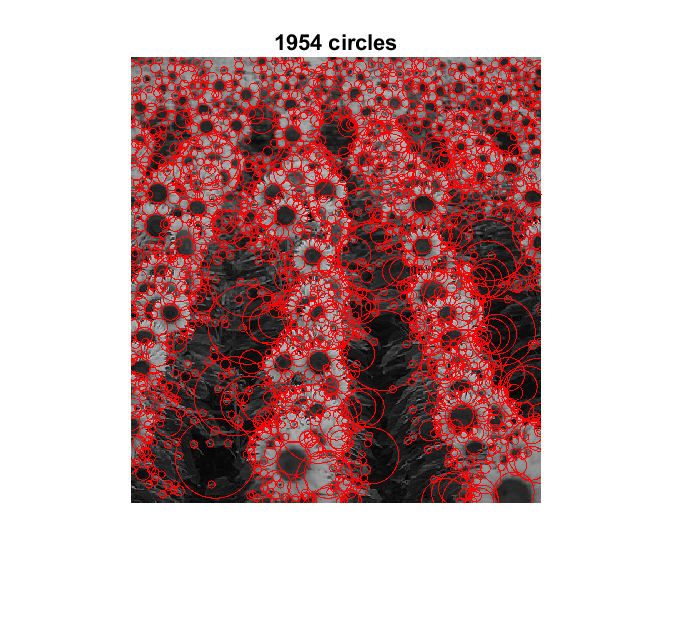
\includegraphics[width=\textwidth]{res/sunflowers_blob_method2.eps}	
			\caption{\tl{Image Downsampling}}	
		\end{subfigure}%
		\begin{subfigure}[b]{0.37\textwidth}
			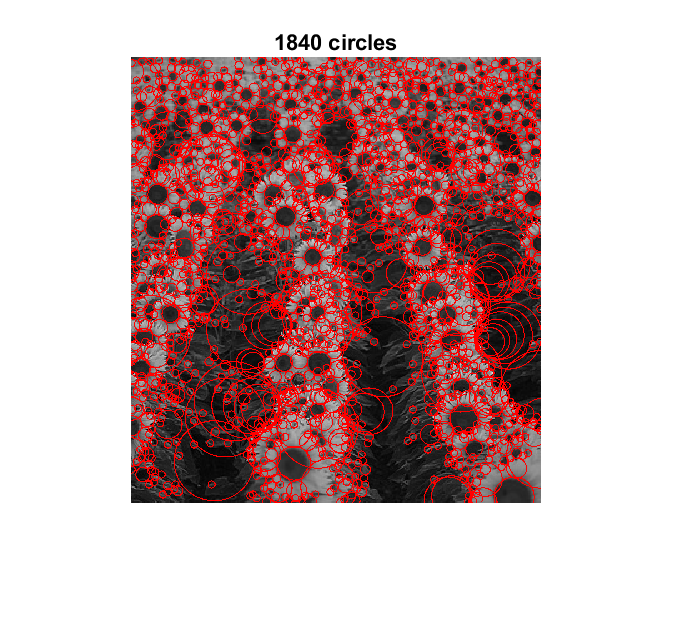
\includegraphics[width=\textwidth]{res/sunflowers_blob.eps}	
			\caption{\tl{Filter Resizing}}	
		\end{subfigure}%	
	\end{figure}
	\begin{table}[!ht]  
		\centering
		\begin{tabular}{|c|c|c|c|c|}
			\cline{2-5}
			\multicolumn{1}{c|}{} & \tl{Butterfly} & \tl{Fishes} & \tl{Snowflakes}  & \tl{Sunflowers}\\ \hline
			\tl{Image Downsampling} & 0.362362  & 0.393882  & 0.221580 & 0.265076  \\ \hline
			\tl{Filter Resizing} & 1.024760 & 1.042106  & 0.706753 & 0.749725 \\ \hline
		\end{tabular}
		\caption{Χρόνοι εκτέλεσης σε \tl{seconds}}
	\end{table}
	\pagebreak	
	\noindent
	Οι κύριες διαφορές μεταξύ των δυο υλοποιήσεων είναι η χρονική πολυπλοκότητα και η διαφορά στον αριθμό των συνολικών \tl{key points.}\\\\
	\noindent
	Πιο συγκεκριμένα, η χρονική πολυπλοκότητα είναι σημαντικά μικρότερη στην περίπτωση που κάνουμε \tl{downsample} την εικόνα και οφείλεται στο γεγονός πως 
	σε αυτή τη μέθοδο σε κάθε \tl{scale} μειώνεται το \tl{size} της εικόνας, ενώ παραμένει σταθερό το \tl{size} του φίλτρου με αποτέλσμα οι πράξεις που απαιτούνται 
	για τη συνέλιξη να μειώνονται σε κάθε στάδιο.\\\\
	\noindent
	Αντιθέτως, στο \tl{Filter Resizing} η εικόνα παραμένει σταθερή ενώ το μέγεθος του φίλτρου αυξάνει σε κάθε \tl{scale} και κατ' επέκταση το μέγεθος της
	συνέλιξης αυξάνει σταδιακά. Επιπλέον, τα υπόλοιπα βήματα του αλγορίθμου \tl{SIFT} για τη εύρεση των μεγίστων και το σχεδιασμό των κύκλων είναι κοινά και στις δυο περιπτώσεις.\\\\
	\noindent
	Επιπρόσθετα, το πλήθος των κύκλων ανάμεσα στις δύο μεθόδους που υλοποιήσαμε διαφέρει. Ειδικότερα, παρατηρούμε ελαφρώς περισσότερους κύκλους στην περίπτωση που 
	κάνουμε \tl{downsample} την εικόνα κατά την κατασκευή του \tl{scale space}. Παράλληλα, βλέπουμε ότι στην δευτερή μέθοδο έχουμε κύκλους με μεγαλύτερη ακτίνα στη 
	θέση κάποιων κύκλων με μικρότερη ακτίνα. Το γεγονός αυτό συμβαίνει καθώς όσο αυξάνουμε το $\sigma $ έχουμε αύξηση του μεγέθους της Γκαουσιανής καμπάνας. \\\\
	\noindent
	Τέλος, με βάση τη χρονική πολυπλοκότητα και τον αριθμό των \tl{key points}, θα επιλέγαμε τη μέθοδο που κάνει \tl{image downsampling}.
\end{document} 